% !TeX program = lualatex
% !TeX root = luaking.tex
% !TeX encoding = UTF-8
% !TeX spellcheck = cs_CZ
%---------------------------------------------------------------------------------------------------
% file fey1ch19.tex
%---------------------------------------------------------------------------------------------------
%=========================== Kapitola: Hmotný střed; Moment setrvačnosti ==========================
\setchaptertoc
\chapter{Hmotný střed; Moment setrvačnosti}\label{fyz:IchapXIX}
  \section{Vlastnosti hmotného středu}\label{fyz:IchapXIXsecI}
    V přecházející kapitole jsme zjistili, že, působí-li velmi mnoho sil na složitou soustavu
    částic, ať už jde o tuhé těleso, pružné těleso, hvězdný oblak nebo něco jiného, a sečteme-li
    všechny tyto síly (jsou to samozřejmě vnější síly, neboť vnitřní síly se vzájemně vyrušily) a
    díváme se na celý soubor částic jako na jedno těleso s celkovou hmotností \(M\), pak „uvnitř“
    existuje takový bod - hmotný střed (\emp{těžiště}) -, že výslednice vnějších sil působí taková
    zrychlení tohoto bodu, jakoby v něm byla soustředěna celá hmotnost souboru. Zabývejme se nyní
    hmotným středem trochu podrobněji.
    
    \begin{figure}[ht!] %\ref{fyz:fig402}
      \centering
      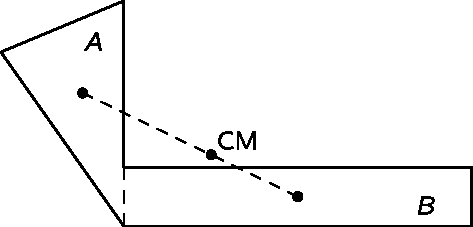
\includegraphics[width=0.3\linewidth]{fyz_fig402.pdf}
      \caption{Hmotný střed složeného tělesa leží na přímce spojující hmotné středy obou částí
              (\cite[s.~260]{Feynman01})}
      \label{fyz:fig402}
    \end{figure}
  \section{Poloha hmotného bodu}\label{fyz:IchapXIXsecII}
  \section{Určení momentu setrvačnosti}\label{fyz:IchapXIXsecIII}
  \section{Kinetická energie rotace}\label{fyz:IchapXIXsecIV}
  \section{Příklady a cvičení}\label{fyz:IchapXIXsecV}



    \begin{figure}[ht!] %\ref{fyz:fig403}
      \centering
      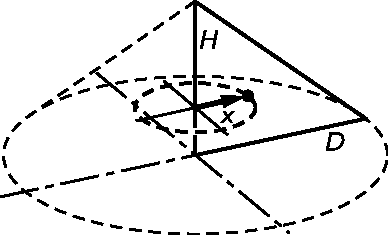
\includegraphics[width=0.3\linewidth]{fyz_fig403.pdf}
      \caption{Pravoúhlý trojúhelník a přímý rotační kužel vytvořený rotujícím trojúhelníkem 
              (\cite[s.~263]{Feynman01})}
      \label{fyz:fig403}
    \end{figure}
    \begin{figure}[ht!] %\ref{fyz:fig404}
      \centering
      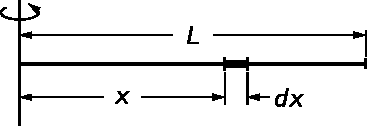
\includegraphics[width=0.3\linewidth]{fyz_fig404.pdf}
      \caption{Přímá tyč \(L\) rotující kolem osy procházející jedním koncem
              (\cite[s.~264]{Feynman01})}
      \label{fyz:fig404}
    \end{figure}

    \begin{figure}[ht!] %\ref{fyz:fig405}
      \centering
      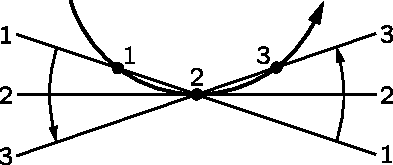
\includegraphics[width=0.3\linewidth]{fyz_fig405.pdf}
      \caption{Tři postupné pohledy na radiálně se pohybující bod na otáčející se podložce
              (\cite[s.~269]{Feynman01})}
      \label{fyz:fig405}
    \end{figure}

  \todo[inline]{Kapitola fey1ch19 je zcela prázdná, pouze obrázky}  
%} %tikzset
%---------------------------------------------------------------------------------------------------